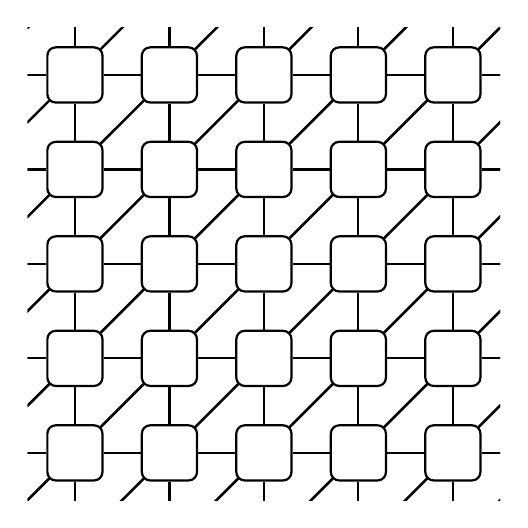
\begin{tikzpicture}[thick]
	
	\def\width{5}
	\def\height{5}
	
	% Space between node centers
	\def\spacescale{1.2}
	
	% Rounding on edges of chips
	\def\rounding{0.7ex}
	
	\pgfmathtruncatemacro{\widthh}{\width-1}
	\pgfmathtruncatemacro{\heightt}{\height-1}
	
	\tikzset{
		chip/.style={draw,rounded corners=\rounding,minimum size=0.7cm}
	}
	
	% Clip off the extra row of chips around the edge that are added to ensure we
	% end up with lots of wires dangling off the edge.
	\clip (-0.5*\spacescale,-0.5*\spacescale) rectangle
	      (\spacescale*\width-0.5*\spacescale,
	       \spacescale*\height-0.5*\spacescale);
	
	% The chips
	\foreach \x in {-1,...,\width}{
		\foreach \y in {-1,...,\height}{
			\node [chip] (chip X\x Y\y) at (\spacescale*\x, \spacescale*\y) {};
		}
	}
	
	% Edge links...
	\tikzset{
		edge wire/.style={}
	}
	
	% The wires
	\foreach \x in {0,...,\width}{
		\foreach \y in {0,...,\height}{
			\pgfmathtruncatemacro{\xx}{\x-1}
			\pgfmathtruncatemacro{\yy}{\y-1}
			
			% South-West to North-East
			\ifthenelse{\xx < 0 \OR \xx = \widthh \OR \yy < 0 \OR \yy = \heightt}{
				\draw [shorten >=-0.5*\rounding,shorten <=-0.5*\rounding]
				      [edge wire]
				      (chip X\x Y\y) to (chip X\xx Y\yy);
			}{
				\draw [shorten >=-0.5*\rounding,shorten <=-0.5*\rounding]
				      (chip X\x Y\y) to (chip X\xx Y\yy);
			}
				
				% South to North
			\ifthenelse{\yy < 0 \OR \yy = \heightt}{
				\draw [edge wire]
				      (chip X\x Y\y) to (chip X\x Y\yy);
			}{
				\draw (chip X\x Y\y) to (chip X\x Y\yy);
			}
				
				% West to East
			\ifthenelse{\xx < 0 \OR \xx = \widthh}{
				\draw [edge wire]
				      (chip X\x Y\y) to (chip X\xx Y\y);
			}{
				\draw (chip X\x Y\y) to (chip X\xx Y\y);
			}
		}
	}
	
\end{tikzpicture}
